%%
%%  This is a LaTeX template for an astronomy Bachelor's thesis.
%%
%%  Version 1.0
%%
%%  Authors: Anders Johansen, Sofia Feltzing, Johan Bijnens (2014)
%%  Send feedback to Anders Johansen <anders@astro.lu.se>
%%
\documentclass[12pt]{report}

\usepackage{a4wide}
\usepackage{graphicx}
\usepackage{natbib}
\usepackage[T1]{fontenc}  
\usepackage[utf8]{inputenc} 
\usepackage{geometry}
\usepackage[justification=centering]{caption}
\usepackage{subcaption}

\usepackage{fancyhdr}
\usepackage{lastpage}
\usepackage{pdfpages}
\usepackage{url}

\pagestyle{fancy}
%\rhead{}
%\chead{}
%\lhead{}
%\rfoot{}
\cfoot{\thepage}
%\lfoot{}

\newcommand{\apj}{ApJ}
\newcommand{\apjs}{ApJS}
\newcommand{\apjl}{ApJ}
\newcommand{\mnras}{MNRAS}
\newcommand{\aap}{A\&A}
\newcommand{\aj}{AJ}
\newcommand{\nat}{Nature}
\newcommand{\pre}{Phys.~Rev.~E}
\newcommand{\araa}{ARA\&A}
\newcommand{\icarus}{Icarus}

\begin{document}

\title{\huge \bf Multiplanetary Systems from Simulated TESS Transit Timing Variations\footnote{This is just a very basic cover page produced by LaTeX -- when
the thesis is done you can get a more formal cover page from Eva Jurlander.}}
\author{Lucas Hellström}

\thispagestyle{empty} % do not count pages just yet

\maketitle

\newpage

\thispagestyle{empty}

\begin{center}
  (this page will contain some more official information in the final version)
\end{center}

\newpage

\thispagestyle{empty}

\begin{center}
  {\bf Abstract}
\end{center}
The abstract is a short summary describing the content of the main text. This
should give enough information about the contents to decide for the intended
audience whether further reading will be useful. The size should be about half
a page, best written at the end, after most of the thesis is written.

\newpage

\thispagestyle{empty}
\mbox{} % this is how we create an empty page in LaTeX

\newpage

\thispagestyle{empty}

\begin{center}
  {\bf Popul\"arvetenskaplig beskrivning}
\end{center}
	När vi letar efter exoplaneter finns det ett antal olika metoder för att hitta dem. Den mest framgångsrika är transitmetoden där ljusstyrkan hos en stjärna studeras under en längre tid. När en planet passerar mellan sin stjärna och en observatör kan en minsking i stjärnans ljusstyrka ses. Uppreras detta i regelbunda intervall kan slutsatsen att det finns en planet runt stjärnan. Genom att studera minskningen i ljusstyrka kan storleken på planeten beräknas vilket kombinerat med massan som fås av andra metoder ger en insikt i hur och vad planeter är uppbygd av. En transit är detta fenomen då en planet passerar mellan stjärnan och en observatör.
	
	Genom att jämföra tiden mellan varje transit för en planet kan ibland variationer ses. Detta beror på att det finns fler planeter runt stjärnan som med hjälp av gravitationskraften accelererar eller decelerera planeten som bevakas. Detta resulterar i att det är möjligt att hitta planeter som i andra metoder är osynliga. 
	
	Keplerteleskopet är ett rymdbaserat teleskop som använder transitmetoden för att hitta exoplaneter. Det har sedan 2009 hittat över 1000 bekräftade exoplaneter vilket gör den till det hittils mest framgångsfulla upgradet i jakten på exoplaneter. TESS, vilket står för Transiting-Exoplanet Survet Satellite, är ett teleskop som sköts upp den 18de april 2018 och använder transitmetoden för att hitta exoplaneter. TESS kommer bli det första rymdbaserade teleskopet att studera hela himlen och kommer observera över 200 000 stjärnor under uppdragets urspungliga längd på två år.
	
	Detta projekt kommer använda data från Keplerteleskopet och simulera data från TESS för att sedan använda den datan för att leta efter TTV. Detta ska ge en uppfattning om hur många system har fler än en planet och resultatet kommer kunna ses som en katalog över multi-planet system vilket kan underlätta framtida forskning där en katalog av detta slag kan vara till användning.
	
	


%This is meant to be popular {\it introduction to} and {\it description of} your
%thesis, preferably written in Swedish. The name is unfortunately misleading. It
%is not a summary but mainly an introduction to what you have done. A good idea
%is to write this when you are about one third through the time allotted for the
%thesis work.
%\\ \\
%Especially important here are the context of your project and why this is an
%interesting project to do. This should be about half a page as well.
% Swedish letters: \"a, \"o, \aa

\newpage

\thispagestyle{empty}
\mbox{} % make sure that TOC starts on a right page

\newpage

\setcounter{page}{1} % start counting pages

\tableofcontents

\newpage

\listoffigures 
\listoftables

\newpage

\chapter{Introduction}

This document is meant as a technical tutorial for writing an
astronomy/astrophysics thesis in LaTeX. Detailed rules about the {\it contents}
of the thesis (Bachelor's thesis or Master's thesis) can be found at the course
websites.

\section{Transits}
	A planet in orbit around it's host star may sometimes cross the line of sight of an observer. When this happens a slight decrease in the stars brightness can be measured. This is called a transit and is today used as a main method to discover exoplanets. From transits the radius of the planet can be determined but it can also be used to find additional planets around the host star which may not be transiting. This will be discussed in section \ref{sec:trans_vari}. With the radius known from the transit method and the mass obtained from different methods such as, for example the radial velocity method, the density of the planet can be calculated. The density is important to understand what the planet is made of and the structure of it.

\subsection{Variations}
\label{sec:trans_vari}

	When measuring the time of one transit one may discover variations in the period which are called Transit-Timing Variations or TTVs. These variations arise from another planet in the system whose gravitational pull accelerates or decelerate the observed planet which results in increased or decreased transit times. An advantage of studying transits in search for TTVs is that planets which does not transit their star can be discovered through TTVs \citep{0004-637X-777-1-3}. As most planets does not transit their star this can increase the number of known exoplanets drastically.

\section{Kepler}
	The Kepler satellite launched in spring 2009 on a mission to study stars in a small patch in the sky to discover Earth-sized exoplanets within the habitable zone, where liquid water can exist on the planetary surface. The brightness of a large amount of stars are measured and then analyzed in order to detect transiting exoplanets.
	
	Kepler started by looking at a very small patch of the sky but in July 2012 one of the four wheels used to keep the patch in focus broke. The telescope requires at least three wheels to function which kept the mission alive. In May 2013 a third wheel failed which resulted in the telescope no longer being able to collect data. The satellite was nonfunctional until the so-called "Second Light (K2)" in early 2014. This mission would use the telescopes remaining two wheels to study stars over a much larger area but for shorter periods.
	
	According to \cite{kepler_num_planet} Kepler found over 2300 confirmed exoplanets and about 2200 candidates which require further studies before they can be confirmed during the main mission, before the second wheel broke down. Since the start of K2 about 300 exoplanets have been confirmed and close to 500 candidate exoplanets. These numbers makes Kepler the most successful exoplanet hunting mission to this date.
	
	
\section{TESS}
	The Transiting Exoplanet Survey Satellite, TESS, is a satellite which were launched on the 18th of April 2018. The satellite is equipped with four cameras which will study the brightness of over 200 000 stars over a two year period. It is the first all-sky transit survey taking place in space.
	
	TESS will study the whole sky by splitting it into 26 sectors, 13 in the southern hemisphere and 13 in the northern hemisphere, which are observed for 27 days each. An illustration of this can be seen in figure \ref{fig:tess_time} where the number of times TESS will observe each sector is shown. TESS will observe the southern hemisphere during the mission's first year, it will then rotate and observe the norther hemisphere for another year.
	\begin{figure}[h!]
	\centering
		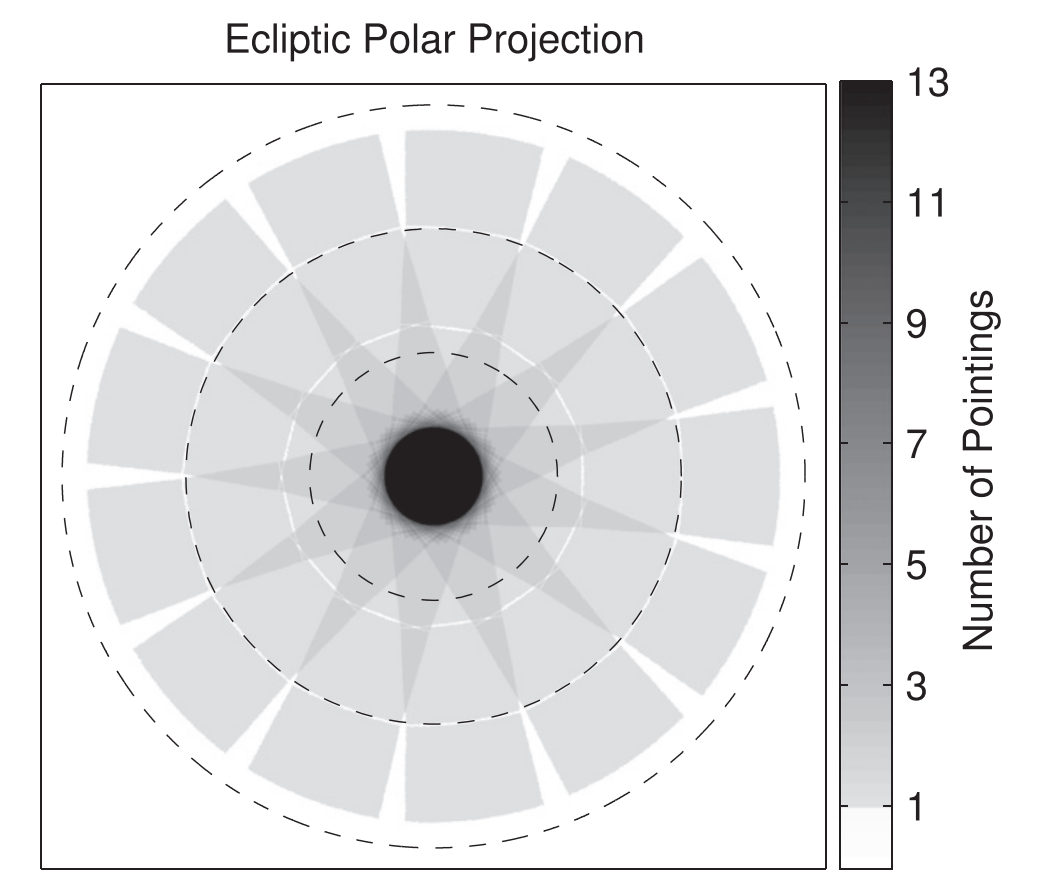
\includegraphics[width=\textwidth]{img/tess_observe_time.png}
		\caption{Illustration of the number of times TESS will observe each sector in the sky.\\ \small{Source: \cite{2015ApJ...809...77S}}}
		\label{fig:tess_time}
	\end{figure}
	
	
\section{TTVFast}
\label{TTVFast_intro}
	TTVFast is a program created by \cite{2014ApJ...787..132D} which simulates planetary systems using an n-body integrator. It requires information about the system in the form of:
	\begin{itemize}
		\item Gravitational constant in $AU^3 \mathrm{day}^{-2}M_{\odot}^{-1}$
		\item Mass of the star 
		
	\end{itemize}
	And also for each planet in the system:
	\begin{itemize}
		\item Period in days 
		\item Eccentricity
		\item Inclination 
		\item Longitude of ascending node, long node for short 
		\item Argument of perihelion, argument for short 
		\item Mean anomaly at the reference time 
	\end{itemize}
	Where Longitude of ascending node and argument of perihelion are orbital elements. The reference time is the time of the start of the integration, in this paper: $t_ref=0$. The program also requires parameters regarding the integration which are given in a setup file:
	\begin{itemize}
		\item Path to file containing info regarding the planets in the system.
		\item Reference time
		\item Time step which is $1/20$ of the period
		\item Final time which in this paper is the duration of the integration
		\item Number of planets
		\item Input flag which specifies in which coordinate system the input parameters are given. This paper uses Jacobi coordinates which relate to a input flag = 0.
	\end{itemize}
	How these parameters are determined and "given" to TTVFast will be discussed in section \ref{simTESS} and \ref{TTVFast_method}.
	
\chapter{Method}
	The code used are written in Python and can be seen in abstract (REF ABSTRACT). It is executed by a bash script which runs the necessary components to create artificial planetary systems, run TTVFast on these systems to generate transit times and then analyze these times in order to find TTVs. These systems are simulated over a long time by the use of WHFast in order to determine the stability of them.

\section{Simulation of TESS objects}
\label{simTESS}
	The bash script starts by running the program to create the artificial systems. By combining data from Kepler obtained from the NASA Exoplanet Archive\footnote{\url{https://exoplanetarchive.ipac.caltech.edu/index.html}} and the results from \cite{2015ApJ...809...77S}, which contains one planet for each system, TESS data are simulated. The planets are separated into two groups based on the effective temperature of their host star. Planets around stars with an effective temperature below 4000 K are put in one group while planets around stars with effective temperature above 4000 K are put into another group. This prevents planets around cold stars to get "matched" with planets around hot stars. 
	
	For each planet in the Sullivan catalogue, a similar planet, in radius and period, are selected from the NASA archive. The ratio of radius and period between the two planets are calculated and multiplied with the Sullivan planets radius and period. This results in that the two planets are identical in radius and period. These ratios are then applied to the rest of the planets in this selected Kepler system to create an artificial system of planets.  
	
	The mass of the planet is required to simulate the system and is approximated using equation \ref{eq:mass_p_low} and \ref{eq:mass_p_high} obtained from \cite{2015ApJ...809...77S}:
	\begin{equation}
	\label{eq:mass_p_low}
	M_p = M_{\oplus} \left[0,440 \left(\frac{R_p}{R_{\oplus}}\right)^3 + 0,614\left(\frac{R_p}{R_{\oplus}}\right)^4\right]
	\end{equation}
	for planets with $R_p < 1,5 \; \mathrm{R_{\oplus}}$ where $R_{\oplus}$ is the radius of Earth and $M_{\oplus}$ is the mass of Earth. For planets with $R_p \geq 1,5$ the equation changes to:
	\begin{equation}
	\label{eq:mass_p_high}
	M_p = 2,69\cdot M_{\oplus}\left(\frac{R_p}{R_{\oplus}}\right)^{0,93}
	\end{equation}
	The mean anomaly is required for each planet and is acquired from the number of transits and the orbital period of the planet. By using a reference point specified when a planet is directly in front the the host star as seen from an observers point of view. This reference point corresponds to a mean anomaly of 90$^{\circ}$ at some time $T_i$, where $i$ is the number of the planet in the system. For a two planet system this means that $M_1=90^{\circ}$ at some time $T_1$ and $M_2=90^{\circ}$ at some time $T_2$. In order to calculate the mean anomaly at some time a time reference point is defined as $t=0$ and the goal is the calculate the mean anomaly of some planet $i$. This can be done by using the mean anomaly at $t = T_i$ and subtracting the number of degrees, $\mathrm{num_{deg}}$, the planet have traveled since then:
\begin{equation}
	M_i(t=0) = M_i(t=T_i) - \mathrm{\#_{deg}}
\end{equation}
	$M_i(t=T_i) = 90^{\circ}$ and the number of degrees traveled is $360^{\circ}$ multiplied by the number of orbits since $t_0$:
\begin{equation}
	M_i(t=0) = 90 - 360\cdot \frac{T_{epoch}}{P_i}
\end{equation}
	where $T_{epoch}$ is the transit epoch and $P_i$ is the period of the planet.
	
	TTVFast also requires inclination, eccentricity, long node and argument. These cannot be simply obtained and need to be assumed. For simplicity the inclination is assumed to be $90^{\circ}$ for all planets which results in the long node to be 0. The eccentricity is obtained from a Rayleigh distribution with mode $\sigma = 0,03$ in order to not get eccentricities above 0.1 as that leads to unstable systems. The argument is obtained from a uniform distribution where $0 < \omega < 360$. The code to obtain the input parameters can be seen in appendix \ref{ap:input_code}. 
	
	How long a system will be observed depends on where in the sky it is located. This time can be obtained from the Web TESS Target tool \footnote{\url{https://heasarc.gsfc.nasa.gov/cgi-bin/tess/webtess/wtm.py}} if the right ascension, RA, and declination, dec, are known. This tool accepts csv files with RA and dec of the systems and outputs the number of times TESS will observe that system. This is then used in the simulation of the systems.
	

\section{TTVFast}
\label{TTVFast_method}
	The next step is to use the systems generated in the previous section and simulate them in TTVFast. The parameters from section \ref{TTVFast_intro} are given to the program to simulate each system. To run TTVFast the parameters are required to be in a specific format and each system requires a setup file mentioned in section \ref{TTVFast_intro}. The bash script creates a new setup file for each system before running the simulation. 

\section{Analyzing results from TTVFast}
	When all systems have been simulated with TTVFast the bash script executes the next part of the program seen in abstract (REF HERE). The transit times need to be corrected as TTVFast outputs the time of a transit. This is done by fitting a linear fit to the times and subtracting this fit. In order to easier see the amplitude of the TTV signals the times are corrected by subtracting the average time from every value which moves the middle of the graph to $y=0$. In order to obtain the amplitude of the TTVs the average of the maximum and minimum transit time are calculated. This is used as the amplitude and the corrected transit times are plotted. \\
	
	In order to further observe interesting systems the position of these systems are required which is obtained from the NASA archive. The positions are given in RA and dec and plotted in a sky map. These coordinates are compensated with Earth's obliquity which is about 23$^{\circ}$. These sky maps are colour coded according to the TTV amplitude and the multiplicity, i.e. the number of planets, of the systems.
\section{Error estimation}
\cite{2005Sci...307.1288H}
	\begin{equation}
		\sigma_t \approx \left[\left(S * t_T\right)^{-1/2} \cdot \left(\frac{R_p}{R_{\star}}\right)^{-3/2}\right] t_T
	\end{equation}
\section{WHFast}
	The artificial systems that are created need to be checked for stability to determine if the assumptions and method of creating them results in realistic and stable systems. For this Rebound \citep{2012A&A...537A.128R}, more specifically the WHFast integrator \citep{2015MNRAS.452..376R}, is used. WHFast is a Wisdom-Holman integrator used for long duration planetary system simulations. For some systems close-encounters occur, WHFast is not a good integrator for these and therefore if such a system is found it will instead be simulated with IAS15 \citep{2015MNRAS.446.1424R}. IAS15 is another integrator for gravitational dynamics and although slower than WHFast it handles close-encounters better.\\
	
	WHFast requires the semi-major axis of each planet in each system. This is obtained from Kepler's law of periods:
	\begin{equation}
		a^3 = T^2 \Rightarrow a = T^{2/3}
	\end{equation}
		where $a$ is the semi-major axis in AU and T is the period in years. 
		
	As the stability simulations take a long time not all systems can be checked for stability. The first systems are selected by their multiplicity in order to see that at least one system of each multiplicity is stable. Then the Hill radius is calculated for each system:
	\begin{equation}
		r_{Hill} = \frac{a_1 + a_2}{2}\left(\frac{M_1 + M_2}{3M_{\star}}\right)^{1/3}
	\end{equation}
	where $a_{1,2}$ is the semi-major axis of the two inner most planets, $M_{1,2}$ is the mass of the two planets and $M_{\star}$ is the mass of the host star. This radius is then used to calculate the separation:
	\begin{equation}
		\Delta = \frac{a_2 - a_1}{r_{Hill}}
	\end{equation}
	The systems with lowest separation is the systems most probable to be unstable and thus they are simulated for stability.
	
\section{Simulation of Ofir objects}
	A paper written by \cite{2018ApJS..234....9O} simulated objects for TTV signals. In order to determine the precision of the methods used in the paper the systems simulated by Ofir et al. are simulated by the same methods as in this paper. The resulting amplitudes of the TTV signals are compared to those of the Ofir systems The Ofir catalogue gives the Kepler ID of the planets, these are then used to obtain the other planetary parameters from the Nasa Exoplanet Archive. These systems are then simulated with the methods from the previous sections.
	

\chapter{Results}

\iffalse Chapters always start on a new page. The chapter names in the template are just
suggestions. You can name your chapters differently and add more if needed.

\begin{verbatim}

       PROGRAM myfortran

       IMPLICIT NONE

       REAL*8 mag(20)
       REAL flux(20)
       INTEGER nstar

       WRITE(*,*) "This program calculates a magnitude"
       READ(*,*) flux(1)
       mag(1)=-2.5*LOG(flux(1))

\end{verbatim}

\fi




\section{Simulated TESS objects}
	The planetary radius of the artificial systems are plotted against the orbital periods in figure \ref{fig:RP_plot_temp_multi}. In the left panel the effective temperature of the host star is represented with a colour map and in the right panel the multiplicity of the system are represented with colour and shape. As can be seen in the left panel most of the measured planets orbit a hot star above 5000 K. The right panel shows that most systems consists of two or three planets. Systems containing five or six planets are few. Both panels show that most of the planets are smaller than earth and have a far shorter period. Short period planets are far easier to discover when using the transit method as it allows for more opportunities to measure the transit.

\begin{figure}[h!]
 	 \centering
 	 \begin{minipage}{.5\textwidth}
 	 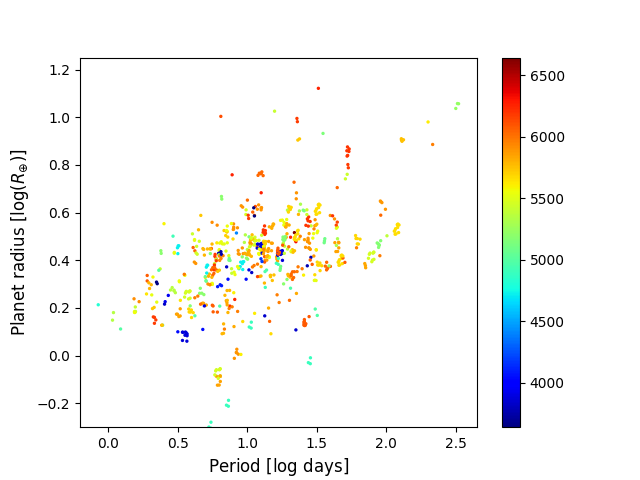
\includegraphics[width=1\linewidth]{img/R_P-plot_effTemp_cut-off.png}


 	 \end{minipage}%
	\begin{minipage}{.5\textwidth}
 	 \centering
 	 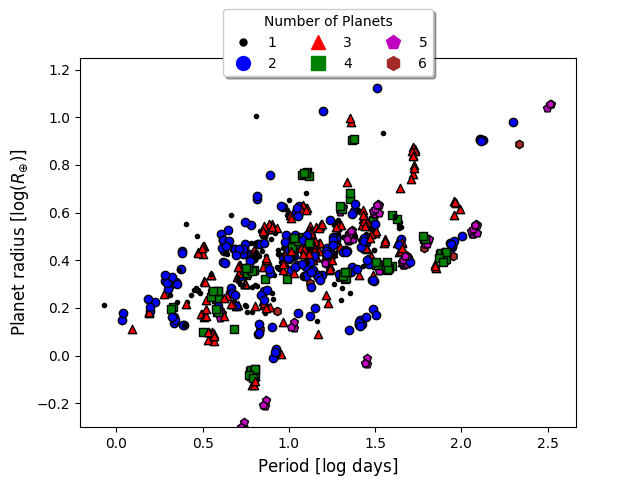
\includegraphics[width=1\linewidth]{img/R_P-plot_numP1.png}
 	 

 	 \end{minipage}
 	  	 \caption{Radius distribution as a function of period for the simulated TESS objects where the colour corresponds to the effective temperature of the host star (left panel) and the colour and shape corresponds to the multiplicity of the system (right panel).}
 	  	 \label{fig:RP_plot_temp_multi}
\end{figure}
	\newpage Figure \ref{fig:skymap_TESS} shows a sky map of the simulated TESS objects and the number of times they are observed. \textit{more comments on this picture when the final version of the picture is done}

\begin{figure}[h!]
	\centering
	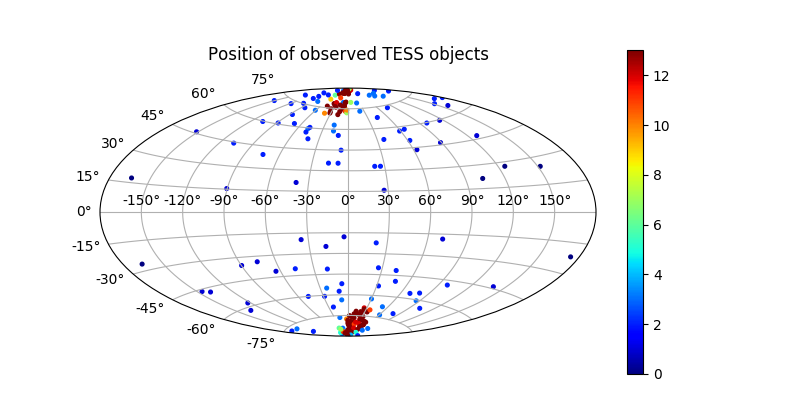
\includegraphics[width=\textwidth]{img/skymap_TESS_wrap.png}
	  \caption{Position of each observed objects colour-coded to show the number of times the object is observed.}	
	  \label{fig:skymap_TESS}	
\end{figure}\newpage
	  


\section{TTV signals from TESS objects}
	Figure \ref{fig:TTV1} shows an example of a TTV signal where the variation is clearly visible. The zero level corresponds to the average transit time in order to see the variations more clearly. The distribution of TTV amplitudes are found in figure \ref{fig:ampl_histo} where amplitudes below 1 minute are filtered out as otherwise they dominate the histogram. It is easy to see that low or no TTV signals dominate but there are some planets showing substantial TTV signals. The location in the sky of these objects are shown in figure \ref{fig:skymap_amp}.
\begin{figure}[h]
 	 \centering
	  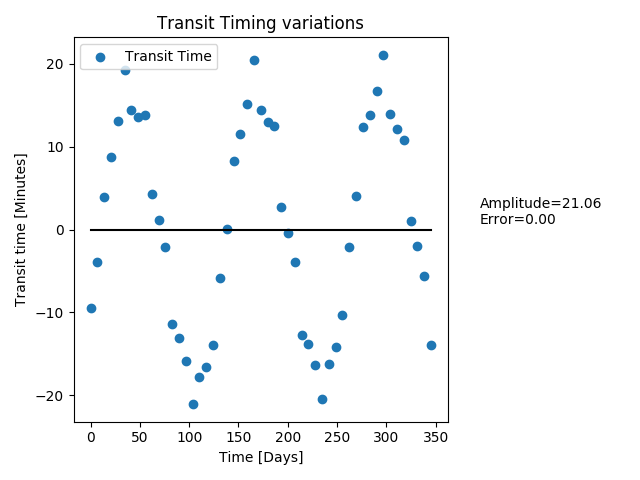
\includegraphics[width=\textwidth]{img/215_1.png}
	  \caption{TTVs as a function of time. The zero level corresponds to average transit time.}
	 \label{fig:TTV1}
\end{figure}
\begin{figure}[h!]
 	 \centering
	  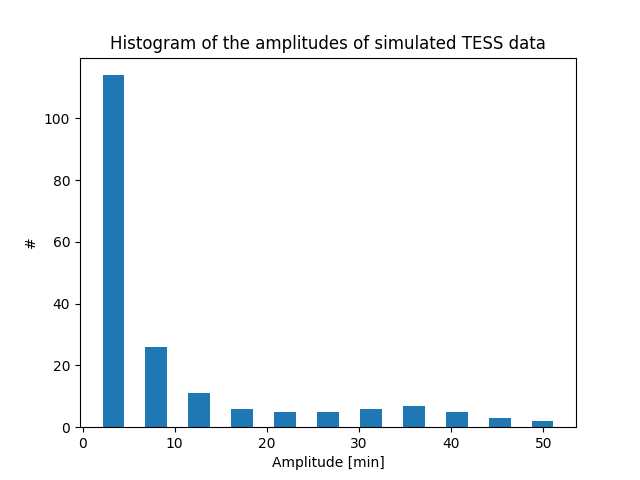
\includegraphics[width=\textwidth]{img/ampl_histo2.png}
	  \caption{Distribution of TTV amplitudes from the simulated TESS objects.}
	 \label{fig:ampl_histo}
\end{figure}
\begin{figure}[h!]
 	 \centering
	  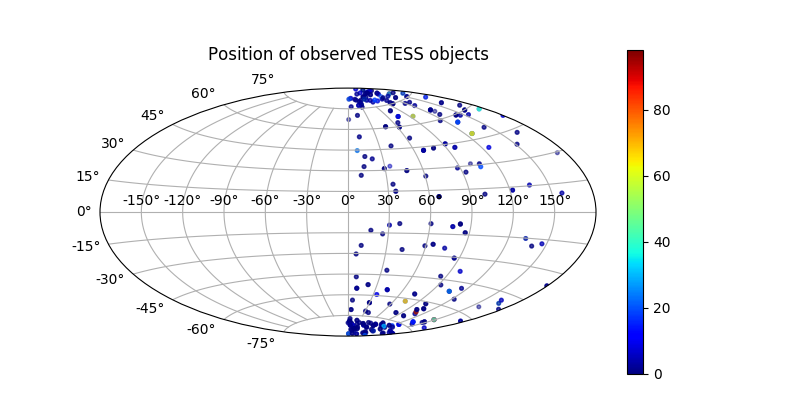
\includegraphics[width=\textwidth]{img/skymap_TESS_wrap_cutoff.png}
	  \caption{Distribution of TTV amplitudes from the simulated TESS objects.}
	 \label{fig:skymap_amp}
\end{figure}
\section{Stability simulations}
	Figure \ref{fig:stability_sim} shows two examples of the results from the stability simulations. For all stability tested systems most of the have not shown any instability. A few systems did eject a planet which  probably is the result of a close encounter. These systems were then re-simulated using IAS15 which showed that they were in fact stable and the ejection was a result from WHFast not being able to handle the close encounters. It can be noted that all of the planets are very close to the host star. This is a result from how the semi-major axis is calculated, as most planets in this paper have a short period the semi-major axis is small which results in very closely packed systems.

\begin{figure}
\centering
\begin{minipage}{.5\textwidth}
  \centering
  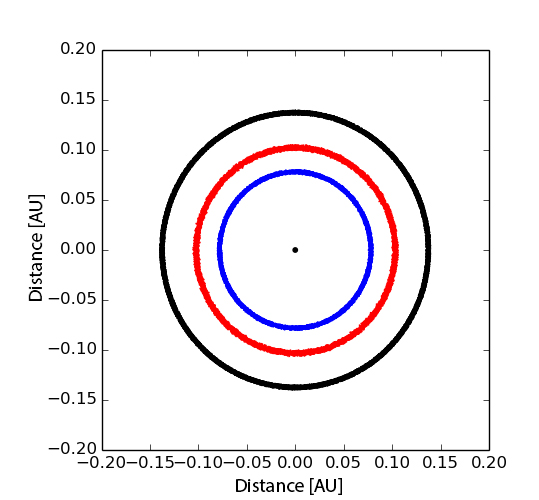
\includegraphics[width=1\linewidth]{img/180.jpg}
 

\end{minipage}%
\begin{minipage}{.5\textwidth}
  \centering
  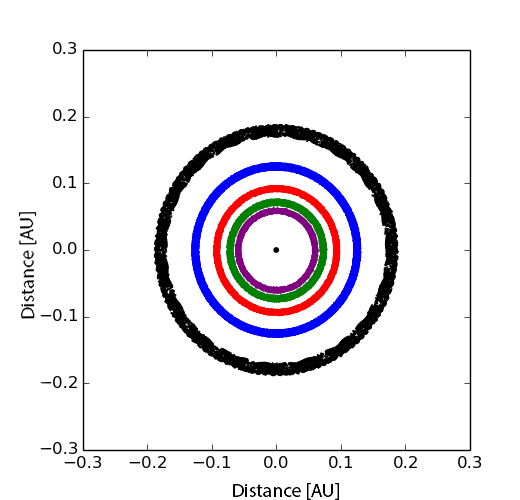
\includegraphics[width=1\linewidth]{img/320.jpg}
  

\end{minipage}
\caption{Orbits of the planets in a three planet system (left panel) and a five planet system (right panel)}
\label{fig:stability_sim}
\end{figure}

\section{Simulations of Ofir systems}
	Figure \ref{fig:ampl_ofir} shows the distribution of TTV amplitudes from the objects from the Ofir catalogue. In this histogram all systems with amplitude below 1 minute are filtered out as they are not of interest in this paper. It is clear that many systems show a small TTV signal but there are a significant portion of systems which show a higher amplitude. The number of systems decreases for higher amplitudes but at amplitudes around 30 minutes the number increases and then decreases for higher amplitude.
\begin{figure}
 	 \centering
	  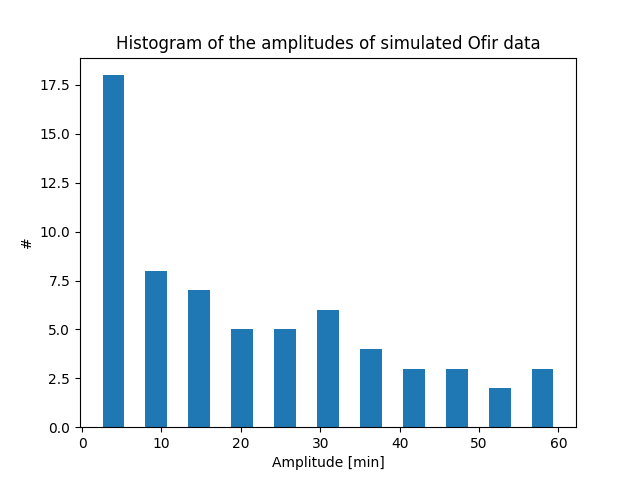
\includegraphics[width=\textwidth]{img/ampl_ofir2.png}
	  \caption{TTV amplitudes of the simulated objects from the Ofir catalogue.}
	 \label{fig:ampl_ofir}
\end{figure}

\iffalse
\begin{figure}
 	 \centering
	  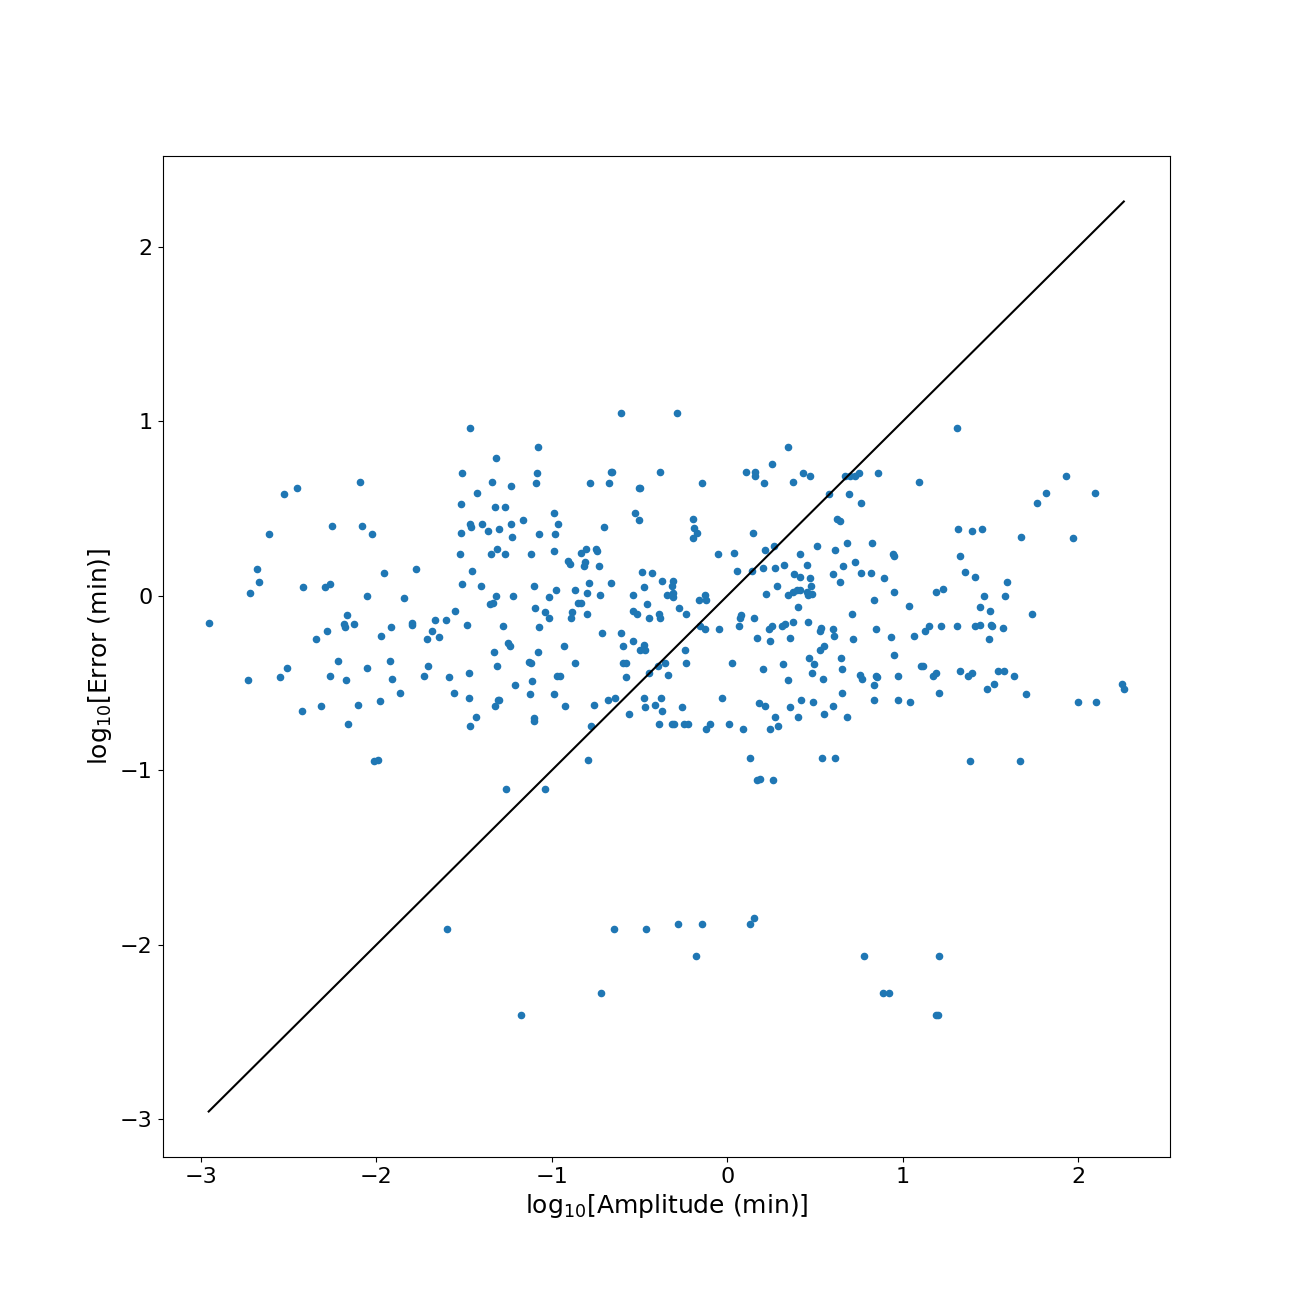
\includegraphics[width=\textwidth]{img/ampErrorLog.png}
	  \caption{Amplitude of the TTV signal as a function of the timing precision.}
	 \label{fig:amp_precision}
\end{figure}

\begin{table}[!h]
\caption{Example table from template}\smallskip
\label{table:1}
\centering  
\begin{tabular}{lrrc}
\hline\hline  
\smallskip
Id of star & I &  V & Var.? \\
\hline
1234 & 15.6 & 17.3 & No \\
5677 & 13.4 & 12.3 & Yes\\
\hline
\end{tabular}
\end{table}
\fi

\chapter{Discussion}
	These results may be used to select systems for further studies. The systems can be observed in more detail by the Characterising Exoplanets Satellite, CHEOPS, or the James Webb telescope. The main difference between these are where in the sky they are able to look at. CHEOPS are not able to measure stars at the poles and are limited to the sky around the plane of Earth's orbit. As TESS will have coverage of the poles for the whole year many of the discovered systems will be at the poles. The James Webb telescope on the other hand will be able to look at the poles. This makes James Webb a very good option for further studies of the TESS objects. 
	
	The artificial systems created in this paper contain some planets which show strong TTV signals, mainly positioned in the ecliptic poles as the systems positioned here are observed for a whole year which gives many more opportunities to detect TTVs. The shape of the histogram in figure \ref{fig:ampl_ofir} are the same as in the Ofir paper. This shows that the methods of simulating systems used in this paper are viable and give reasonable results. (\textbf{reason for increase at 30min?})
	
	The way of determining the amplitude of the TTVs are very simplistic. It is simply an average of the highest and lowest value. This can be improved by some kind of fit as the TTV signals are often in the shape of a sine curve but due to time constraints this paper does not include this way of determining the amplitude.
	
	Using WHFast, most systems tested for stability show no sign of instability. The few that do are simulated using IAS15 where they are shown to be stable and the instability from WHFast can be considered an affect of WHFast's inability to handle close encounters.
	
	(\textit{something about the errors, not included as the error bars are currently not correct})
\chapter{Conclusions}


\section*{Acknowledgements}

Simulations in this paper made use of the REBOUND code which can be downloaded freely at \url{http://github.com/hannorein/rebound}.\vspace{0.5cm}\\
This research made use of Astropy, a community-developed core Python package for Astronomy (Astropy Collaboration, 2013).

%\bibliographystyle{natbib}
%\begin{thebibliography}{99}
%\bibitem[Alexander \& Armitage(2007)]{2007MNRAS.375..500A}
%  Alexander, R.~D., \& Armitage, P.~J. 2007, \mnras, 375, 500
%\bibitem[Santos et~al.(2001)Santos, Israelian, \& Mayor]{2001A&A...373.1019S}
%  Santos, N.~C., Israelian, G., \& Mayor, M. 2001, \aap, 373, 1019
%\end{thebibliography}

\bibliographystyle{aa}
\bibliography{references}

\begin{appendix}

\chapter{This is an appendix}
\label{ap:input_code}
You can put long mathematical derivations or tables in appendices.

\chapter{This is another appendix}

\end{appendix}

\end{document}
